
%{{{
\documentclass[a4paper,12pt]{article}
\usepackage{fullpage}
\usepackage[T1]{fontenc}
\usepackage{amsmath}
\usepackage{amssymb}
\usepackage[utf8]{inputenc}
\usepackage{color}
\usepackage{authblk}
\usepackage{todonotes}
\usepackage{caption}
\usepackage{url}
\usepackage{float}
\usepackage{sectsty}
\usepackage{pdfpages}
\usepackage[section]{placeins}
\DeclareCaptionFont{white}{\color{white}}
\DeclareCaptionFormat{listing}{\colorbox{gray}{\parbox{\textwidth}{#1#2#3}}}
\captionsetup[lstlisting]{format=listing,labelfont=white,textfont=white}
\usepackage{setspace}
\usepackage[toc,page]{appendix}
\usepackage{framed}
\usepackage{geometry}

\usepackage{alltt}
\usepackage{subfig}

% Change section fonts
\allsectionsfont{\sffamily}

% For code box
\usepackage{xcolor}
\usepackage{listings}
\usepackage{caption}
\DeclareCaptionFont{white}{\color{white}}
\DeclareCaptionFormat{listing}{%
  \parbox{\textwidth}{\colorbox{gray}{\parbox{\textwidth}{#1#2#3}}\vskip-4pt}}
  \captionsetup[lstlisting]{format=listing,labelfont=white,textfont=white}
  \lstset{frame=lrb,xleftmargin=\fboxsep,xrightmargin=-\fboxsep}
% End code box

\usepackage{cite}

% General parameters, for ALL pages:
\renewcommand{\topfraction}{0.9}	% max fraction of floats at top
\renewcommand{\bottomfraction}{0.8}	% max fraction of floats at bottom
% Parameters for TEXT pages (not float pages):
\setcounter{topnumber}{2}
\setcounter{bottomnumber}{2}
\setcounter{totalnumber}{4} % 2 may work better
\setcounter{dbltopnumber}{2} % for 2-column pages

\addtolength{\topmargin}{0.5in}

\usepackage{fancyvrb}
\usepackage{titlesec}


\usepackage{tikz} \usetikzlibrary{trees}
\usepackage{hyperref} % should always be the last package

% subsubsubsection
\titleclass{\subsubsubsection}{straight}[\subsection]

\newcounter{subsubsubsection}[subsubsection]
\renewcommand\thesubsubsubsection{\thesubsubsection.\arabic{subsubsubsection}}
\renewcommand\theparagraph{\thesubsubsubsection.\arabic{paragraph}} % optional; useful if paragraphs are to be numbered

\titleformat{\subsubsubsection}
{\normalfont\normalsize\bfseries}{\thesubsubsubsection}{1em}{}
\titlespacing*{\subsubsubsection}
{0pt}{3.25ex plus 1ex minus .2ex}{1.5ex plus .2ex}

\makeatletter
\renewcommand\paragraph{\@startsection{paragraph}{5}{\z@}%
    {3.25ex \@plus1ex \@minus.2ex}%
    {-1em}%
{\normalfont\normalsize\bfseries}}
\renewcommand\subparagraph{\@startsection{subparagraph}{6}{\parindent}%
    {3.25ex \@plus1ex \@minus .2ex}%
    {-1em}%
{\normalfont\normalsize\bfseries}}
\def\toclevel@subsubsubsection{4}
\def\toclevel@paragraph{5}
\def\toclevel@paragraph{6}
\def\l@subsubsubsection{\@dottedtocline{4}{7em}{4em}}
\def\l@paragraph{\@dottedtocline{5}{10em}{5em}}
\def\l@subparagraph{\@dottedtocline{6}{14em}{6em}}
\newenvironment{custommargins}[2]%
  {\addtolength{\leftskip}{#1}\addtolength{\rightskip}{#2}}{\par}
\makeatother

\setcounter{secnumdepth}{4}
\setcounter{tocdepth}{4}

% useful colours (use sparingly!):
\newcommand{\blue}[1]{{\color{blue}#1}}
\newcommand{\green}[1]{{\color{green}#1}}
\newcommand{\red}[1]{{\color{red}#1}}

% useful wrappers for algorithmic/Python notation:
\newcommand{\length}[1]{\text{len}(#1)}
\newcommand{\twodots}{\mathinner{\ldotp\ldotp}} % taken from clrscode3e.sty
\newcommand{\Oh}[1]{\mathcal{O}\left(#1\right)}

% useful (wrappers for) math symbols:
\newcommand{\Cardinality}[1]{\left\lvert#1\right\rvert}
\newcommand{\Ceiling}[1]{\left\lceil#1\right\rceil}
\newcommand{\Floor}[1]{\left\lfloor#1\right\rfloor}
\newcommand{\Iff}{\Leftrightarrow}
\newcommand{\Implies}{\Rightarrow}
\newcommand{\Intersect}{\cap}
\newcommand{\Sequence}[1]{\left[#1\right]}
\newcommand{\Set}[1]{\left\{#1\right\}}
\newcommand{\SetComp}[2]{\Set{#1\SuchThat#2}}
\newcommand{\SuchThat}{\mid}
\newcommand{\Tuple}[1]{\langle#1\rangle}
\newcommand{\Union}{\cup}

\newcommand{\fix}{\colorbox{yellow!30}{TODO:}}

\usetikzlibrary{positioning,shapes,shadows,arrows}
\providecommand{\keywords}[1]{\textbf{\textit{Keywords: }} #1}

%}}}
\title{\textbf{Designing a Virtual Security Management Layer for Cloud Content}}
\author{Lukas Klingsbo}



%{{{
\begin{document}

\maketitle
%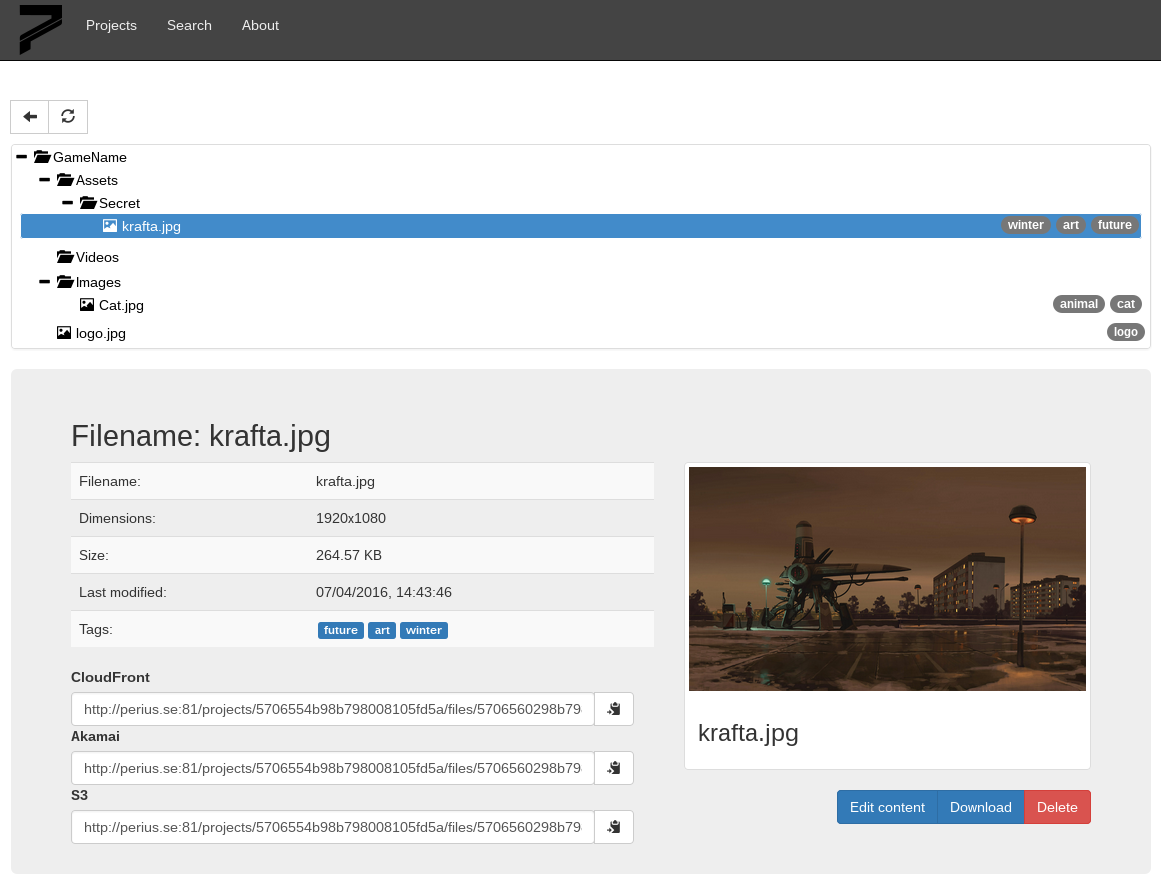
\includepdf[pages={1}]{front.pdf}
%\thispagestyle{empty}
%\newpage\null\thispagestyle{empty}\newpage

\pagenumbering{roman}
\setcounter{page}{1}

%\includepdf[pages={1}]{abstract.pdf}

%}}}
\begin{abstract}
    \fix Abstract is written last

\keywords{}
\end{abstract}

%{{{
\newpage\null\thispagestyle{empty}\newpage

\setcounter{tocdepth}{3}
\tableofcontents

\clearpage
\pagenumbering{arabic}
\setcounter{page}{1}

%}}}
\section{Introduction}
Developing large projects containing static content usually involves using a Content Distribution
Network to be able to scale to a larger user base. The commercial Content Distribution Networks are
usually fairly easy to use, the content that is to be used in a project is usually simply uploaded
and then distributed over the globe when the public requests it. For secret content this can be a
problem and an inconvenience, and that is what this thesis is about. This work examines ways of
enforcing virtual access control on content and groups of content, in the form of containers and
snapshots. A system was developed to make the underlying theory work in practice. 

The research question that this report answers is how and whether it is practically feasible to use
Copy-on-Write for a high-level system like the one that is implemented. 

\fix Clarify problem definition and research questions
\newpage
\section{Background}
\subsection{About Uprise}
Uprise (formerly known as ESN) is a company based in Uppsala, Sweden. It is an EA studio focussing 
on creating great gaming experiences, which means that they are mostly not focussed on the actual 
gameplay which other EA studios like DICE is. Currently Uprise has a lot of focus on developing 
companion apps and a new form of menu systems.

\subsection{Prior Work}
\subsubsection{Copy-on-Write}
This work relies heavily on the Copy-on-Write principle, which was founded and used in the Mach
kernel~\cite{COPYONWRITE}, as it can be used to efficiently create snapshots and help solving
concurrency problems that otherwise can occur.

Copy-on-Write is used in for example virtual memory management systems~\cite{VIRTCOW}, snapshot
algorithms and as an optimisation technique for objects and types in several programming
languages\cite{LANGCOW}.

Its principle is that when processes or nodes share data in between each other, the data is not
copied until one of the processes makes changes to it. This is an optimisation as the processes does
not have to send or copy all of the related data that is in memory, rather they only have to send
pointers to the data. After many Copy-on-Write's a complex tree structure can be built up, but
optimisations can be done to simplify that structure~\cite{COPYONWRITE2}.

\fix Polish and extend

\newpage
\section{Related Terminology}
\subsection{Abbreviations}
\subsubsection{JPF}
Java Path Finder - It was developed by NASA and in 2005 they released it under an open source
licence, which made more people contribute to the project. JPF is usually used for doing model
checking of concurrent programs to easily find for example race conditions and dead locks.

\subsubsection{CDN}
Content Distribution/Delivery Network - Replicates content to several servers, usually spread out
geographically. Once a request is made, the network serves content from the server closest to the
requester.

\subsection{Terms}
\subsubsection{Snapshot}
A snapshot is a way to record the full state of a system at a specific time. The term comes from
photography where a photo can be seen as the state of what the photo is of, at a certain time.
Snapshots should not be confused with a full copy of a system, or part of a system, as full copies 
can be used as backups meanwhile snapshots are not very effective means of backup in the case of 
data corruption. It is not effective against data corruption as snapshots usually still refer to 
unchanged data that is still a part of the system~\cite{SNAPSHOT}.

\newpage
\label{sec:model}
\section{Model}
The model for this work should show how the data can not be accessed or modified by unauthorized
users and how the integrity of the data is always kept in the Perius system. 

There could also be another relevant part included in the model, to show that content can not be 
accessed by unauthorized viewers once the content is uploaded to a CDN. But as that should already 
have been thoroughly checked by the CDN providers this work can focus solely on the internal users 
and content of the management system. 

\subsection{Related work}
The model for this paper is based on the work that was done by Bell, D Elliott, LaPadula and Leonard
J in their papers Secure computer systems: Mathematical foundations~\cite{BLP1} and Secure computer
systems: A mathematical model~\cite{BLP2}. In these papers the foundation was laid for how to model
a computer system to be able to analyse the security of a system. Furthermore this paper was also 
inspired by Biba, Integrity considerations for secure computer systems~\cite{BIBA}, where many of 
the points made by him was taken into consideration when inspecting that the integrity of the data 
was always sound.

\subsection{Approach}
\fix Write about how the approach is similar to BLP and that it is not a proof etc

As this work only presents an informal model of how the system is designed it can not be regarded as
a proof for the actual implementation of the system to be flawless. The model should how ever give a 
strong idea of the soundness of the design of the system.

The copy-on-write system is only used for files as all of the other objects in the system is
basically just meta data and not classed as important, from an data integrity point of view, as the 
actual files themselves. 

\subsection{Elements of the Model}
\begin{center}
    \begin{tabular}{ | l | l | l | p{5cm} |}
        \hline
        \textbf{Set} & \textbf{Elements} & \textbf{Semantics} \\ \hline
        C   & $c_0\dots c_n$                & Containers; folders in the virtual file system\\ \hline
        F   & $f_0\dots f_n$                & Files; files, images, videos\\ \hline
        M   & $m_0\dots m_n$                & Content; Meta-data for files\\ \hline
        U   & $u_0\dots u_n$                & Users; registered users in the system\\ \hline
        A   & $A[u_0,c_0]\dots A[u_n, c_n]$ & Access matrix; describes what containers users have access to\\ \hline
    \end{tabular}
\end{center}


\subsection{Access rights}
The \textit{a} notation is meant to symbolise an access token, and if \textit{a} exists in the requested entity of
the matrix the corresponding user to that entity has full access to the corresponding object.

\begin{equation}
    \begin{split}
        u \in U \text{ can read } c \in C & \Iff u \in A[u,c] \\
        u \in U \text{ can write } c \in C & \Iff u \in A[u,c] \text{ and readonly } \notin c \\
        u \in U \text{ can delete } m \in c & \Iff u \in A[u,c] \text{ and readonly } \notin c \\
        u \nexists U \text{ can delete } f \in F \\
        \forall c \in C, \quad \exists u \in U & \mid a \in A[u,c] 
    \end{split}
\end{equation}

% The last one means that no users can delete actual files

\subsection{Data integrity}
A computer system or subsystem is defined as possessing the property of integrity if it behaves consistently
according to a defined standard. This implies that a subsystem possessing the property of integrity
does not guarantee an absolute behaviour of the system, but rather that it performs according to
what its creator intended ~\cite{BIBA}.

\subsection{Initial Assumptions}
To create an integrity model, some initial assumptions have to be made about what the correct behaviour
of the system is, which the model then can be shown to follow. In this work unintentional behaviour
as the result of data modification is the main concern, which could be used for sabotage or simply be the
effect unintentional unfortunate race conditions etc. 

\subsection{Integrity Threats}
According to Biba et. al~\cite{BIBA} one can consider two threat sources, namely subsystem external
and subsystem internal. The external sources could be another system calling the subsystem with
faulty data or trying to make inaccurate calls to program functions, it could also be somebody
trying to tamper with the exposed functions of the program. Threats that are internal could be a
malicious part of the subsystem or simply an incorrect part of the subsystem, which does not behave
according to specification.

In this work external threats are handled as threats that can occur from what has been exposed by
the API (See Section~\ref{sec:API} and internal threats as incorrect implementation. As the server
and its system are assumed safe malicious subsystems are not considered.

\subsection{Consequences of modification} \label{sec:conseq}

\begin{center}
    \begin{tabular}{ | l | l | l | p{5cm} |}
        \hline
        \textbf{Action} & \textbf{Semantics} \\ \hline
        u, read(o)            & User u reads object o\\ \hline
        u, write(o)           & User u writes object o\\ \hline
        u, copy(o)            & User u copies object o and the copy gets a new ID\\ \hline
        u, change(o)          & User u locally changes object o \\ \hline
        u, modify(o', o)      & User u globally modifies object o based on object o'\\ \hline
        u, delete(o)          & User u deletes object o\\ \hline
        u, snapshot(o)        & User u takes a snapshot of object o \\ \hline
    \end{tabular}
\end{center}

\begin{equation} \label{eq:fileupdate}
    \begin{split}
        m' & = u, read(m) \land \\
        x  & = f \in m' \land \\
        f' & = u, change(x) \land \\
        u, & write(f') \land \\
        u, & modify(f', m) \Implies f \in F \land f' \in F
    \end{split}
\end{equation}
If a user wants to update a file in a content, the file is copied and the original is intact.

\begin{equation} \label{eq:contentupdate}
    \begin{split}
        m' & = u, read(m) \land \\
        m'' & = u, change(m') \land \\
        m''' & = u, modify(m'', m) \Implies \\
        m''' & \in M \land m \not \in M
    \end{split}
\end{equation}
If a user reads content and then writes to it, the content is directly changed.

\begin{equation} \label{eq:containerupdate}
    \begin{split}
        c' & = u, read(c) \land \\
        c'' & = u, change(c') \land \\
        c''' & = u, modify(c'', c) \Implies \\
        c''' & \in C \land c \not \in C
    \end{split}
\end{equation}
If a user reads a container and then writes to it, the container is directly changed.

\begin{equation} \label{eq:copy}
    \begin{split}
        & f' = f \in m \\
        & m' = u, copy(m) \Implies \\
        & m' \neq m \land \\
        & f' \in m' \land f' \in m
    \end{split}
\end{equation}
If a user copies a content, the new content is not equals the old (because of its new ID), however
they both refer to the same file.

\begin{equation} \label{eq:snapshot}
    \begin{split}
        s = u, snapshot(c') \Implies \\
        \forall c \in c', u, copy(c) \in s \land \\
        \forall m \in c', u, copy(m) \in s \land \\
        (\forall f \in c' \Implies f \in s)
    \end{split}
\end{equation}
If a user creates a snapshot of a container the full container tree is re-created with new ids and
its content still refers to the same files.

\begin{equation} \label{eq:delete}
    \begin{split}
        f' = f \in (u, read(c)),  \\
        u, delete(c) \Implies \\
        c \not \in C \land f' \in F
    \end{split}
\end{equation}
If a user deletes content, the file referred to in the content is not deleted.

\subsection{Interaction of Multiple Accesses} \label{sec:multiple_access}
\fix Rename consequence?
\\
As a result of consequence~\ref{eq:contentupdate} and~\ref{eq:containerupdate} there can be race
conditions where the last write wins. This could be solved by locks or transactions, but as updates
are not based on each other, the trade-off for this inconsistency to scalability and speed is
intentional. However as can also be seen in consequence~\ref{eq:fileupdate}, if a file is
removed from a content that file is not removed from the set of files, even though its modification
process is not the last one to write to the content. This is necessary as a file can be referenced
from several content and the removal process can not atomically ensure that the file is not referred
to by another content. This results in a lot of files in the system which are not referenced from
anywhere. This can be solved by either making each file keep track of how many times it is referred
to and also make it possible to check this number and delete the file in an atomic fashion. An
easier approach would be to have a garbage collector which locks parts of the system momentarily
meanwhile it removes files which are not referenced.
\\
There is also the chance to have content and containers that are not referenced from anywhere and
result in being garbage in the system. This could happen as a result of consequence~\ref{eq:delete}
in combination with any of the other consequences listed in Section~\ref{sec:conseq}. The basic idea
is that an entity is deleted meanwhile another is created or modified to have that entity as its
parent and thus creating a separate tree that can not be reached from the root node of the project.
These type of inconveniences should also be cleaned up by the garbage collector.

\subsection{Findings}
\fix Add more findings
\subsubsection{Garbage Collection}
For the system to reach the decided eventual consistency~\cite{KLINGSBO}, garbage collection will be
needed. As of the conclusion in Section~\ref{sec:multiple_access} from Section ~\ref{sec:conseq} 
there will be objects in the system that can not be reached and should therefore be cleaned up for 
them not to cause negative performance effects on the system.

\newpage
\section{Implementation}
\subsection{Background}
\subsubsection{The current system} \label{sec:current_system}
Today a system called battlebinary~\cite{BATTLEBINARY} is used for managing and uploading files,
mostly images, to content delivery networks. The current system does not make use out of the
security features that the CDN's are offering, instead it uses a form of security by obscurity. When
a file is uploaded to a CDN it is open for the public, but its filename is composed out of its
original filename concatenated with a part of the MD5 hash of the content of the file, which makes
it an extremely hard process to access the file on the CDN without access to the original file or a
reference to the URI.

In the current system you can only upload a file once as there will be a collision in the upload
otherwise, as the old and the new file will have the same MD5 hash.  

\subsubsection{Problem description}
As the current system does not offer proper security measurements, is lacking a lot of features that
is needed and does not scale very well, a new system should be developed. This work is about
examining a way of implementing Copy-on-Write in a high level system like this, which should solve
the scalability problem and make it possible to implement wanted features like snapshots, cloning
and concurrent modifications of content.

\subsection{Related Technologies}
\subsubsection{React}
React is a JavaScript library for building user interfaces. React uses both its own virtual DOM and
the browser's, this makes it able to efficiently update dynamic web pages after a change of state
through comparing the old virtual DOM with the resulting virtual DOM after the state change and then
only update the browser's DOM according to the delta between the virtual DOMs~\cite{REACT}. React
can be seen as the system for handling views in front-ends implementing a MVC
(Model-View-Controller) architecture.

\subsubsection{Reflux}
Reflux~\cite{REFLUX} is an idea and a simple library of how to structure your application. It
features a unidirectional dataflow (see Figure~\ref{fig:reflux}) which makes it more suitable, than
for example Flux~\cite{FLUX}, when using a functional reactive programming style.

\begin{figure}[htp] 
    \centering
    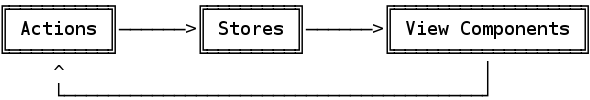
\includegraphics[scale=0.4]{reflux.png}
    \caption{Reflux unidirectional dataflow}
    \label{fig:reflux}
\end{figure}

\subsubsection{Scala} 
Scala is a multi-paradigm programming language. It most commonly runs on the JVM and compared to
Java it supports most functional programming features at the same time as it supports object
oriented programming~\cite{SCALA}.  

\subsubsection{REST} 
REST stands for representational state transfer, it is an architectural idea for writing stateless
services. These services usually use URIs to identify specific resources and HTTP to modify or query
these resources~\cite{REST}. 

\subsubsection{MongoDB}
MongoDB is a document-oriented database which means that it does not have the concept of rows as
normal relational databases has. Instead each entity in the database is stored as a document which
is not fixed to a predefined table structure~\cite{MONGODB}. MongoDB lacks the support for joins to
improve its possibility to scale, which can be a big down side to some applications containing the
need for such logic.

\subsection{Methods for determining\\implementation details}
This chapter introduces the different methods used to determine how the new system should be
implemented, which DBMS it should use and how the estimation of long term scaling was done.

\subsection{Snapshot functionality}
\fix Structure to compare snapshot systems and conclude how Perius snapshot system was designed
\subsubsection{Copy-on-Write}
\label{sec:copy-on-write}
To efficiently create snapshots of a system Copy-on-Write can be used to make it possible to create
snapshots in O(1)\cite{BTRFS}, this is due to the fact that to create a snapshot in a system using
Copy-on-Write you only need to reference the current nodes in the tree and make sure that they are
not removed, see Figure~\ref{fig:btrfs_tree}.

As the persistent storage, used in this implementation (Section~\ref{persistent_storage}), does not
implement transactions or locks a lot of different problems can occur when several clients are
working on the same data set at the same time. Such problems could be race conditions and
determining the happened-before relation. In this work this problem is solved by implementing
Copy-on-Write.
\fix Move last paragraph

\subsubsection{Full Copy}
Full copy or deep copy, as opposed to copy-on-write, is a copy where everything is copied directly
and not only when an object is changed. This is easier to implement but is in most cases more
inefficient as more disk space will have to be used and if used with for example certain tree 
structures the part of the tree that needs to be copied will have to be traversed. 

\subsubsection{Comparison of Copy-on-Write system implementations}
\subsubsubsection{BTRFS}
Btrfs is a B-tree file system for Linux which makes use of Copy-on-Write to make it able to do
efficient writeable snapshots and clones. It also supports cloning of subtrees without having to
actually copy the whole subtree, this is due to the Copy-on-Write effect. As several nodes in the
tree can refer to the same node each node keeps track of how many parents it has by a reference
counter so that the node can be deallocated once the node does not have any parents any more. The
reference counter is not stored in the nodes themselves but rather in a separate data structure so
that a nodes counter can be modified without modifying the node itself and therefore eludes the
Copy-on-Write that would have to occur.

\begin{figure}[htp] \centering{
    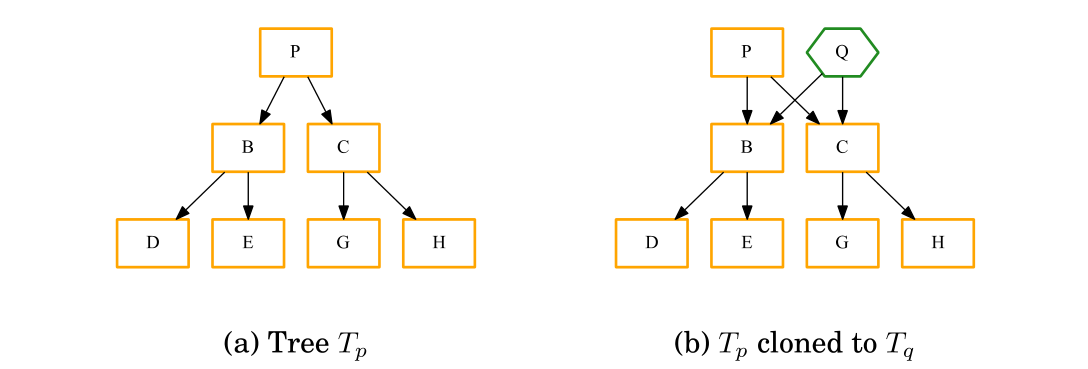
\includegraphics[scale=0.4]{newtree.png}}
    \caption{Cloning mechanism of Btrfs~\cite{BTRFS}}
    \label{fig:btrfs_tree}
\end{figure}

\subsubsubsection{Mach kernel}
In the mid 80's when the development of the Mach kernel started, there was problems with that
physically copying memory was too slow. Too minimise the copying of memory, Copy-on-Write was
implemented. It was implemented so that virtual copy operations could be done and so that tasks
could share read-write memory~\cite{MACH}.


\fix Insert more systems here

\subsubsection{Snapshot functionality of Perius}
In Perius snapshots and clones are not taken in the fashion which Btrfs uses, which can be seen in
Figure~\ref{fig:btrfs_tree}. As Perius does not have the tree structure pre-built and each node is
instead stored in a flat storage space, such operation would be too computationally expensive as
trees would have to be merged when collisions occur, due to the non-blocking nature of the
application. Instead this implementation makes a full copy of the meta-data of the tree, but still
refers to the same binary files until they are changed, which results in the creation of a new node.

\fix Relate section more to comparison

\subsection{Resulting system}
\subsubsection{Perius}
Perius is the implementation that was done to solve the problem at hand at Uprise. Perius has a
back-end written in Scala and a front-end written in Javascript (ES6), but they are both
interchangeable.  The back-end has a REST API running, which is how the front-end communicates with
the back-end.

\fix Picture of the newest front-end
\begin{figure}[htp] \centering{
    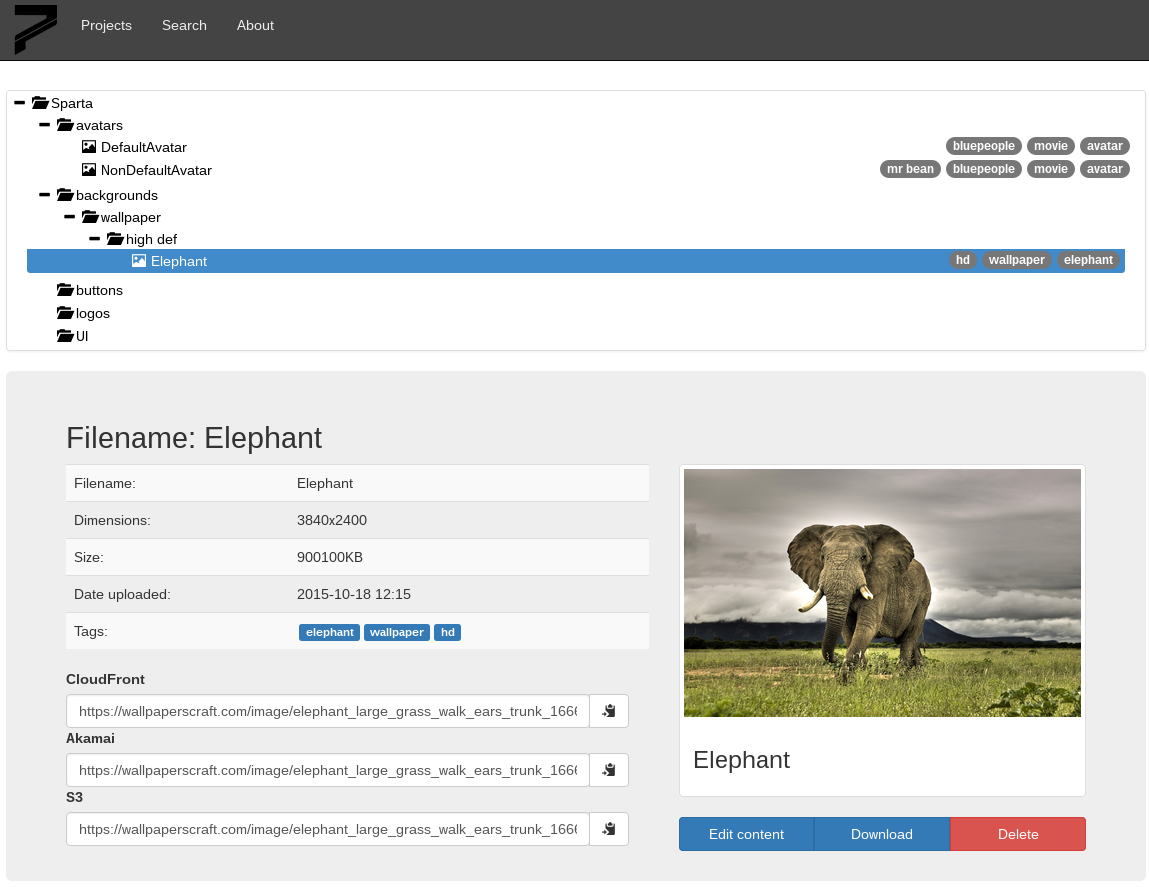
\includegraphics[scale=0.4]{frontend.png}}
    \caption{Front-end~\cite{BTRFS}}
    \label{fig:frontend}
\end{figure}


The service features a virtual file structure over the assets that has been stored, snapshots,
security management of whole containers as well as individual files, audit and access logging, multi
project support and a modular design for persistent storage.

The front-end is written in ES6 with React and Reflux, and the styling is done with the help of
Bootstrap.

\subsubsection{Copy-on-Write}
\fix Rename section and move

This implementation is far from as efficient as the other Copy-on-Write systems described in
Section~\ref{sec:copy-on-write} in most aspects, but more efficient in some. As the implementation
is built upon MongoDB as persistent storage and not a pure tree structure, single nodes can be
fetched in O(1) but when querying for subtrees they need to be built first, which takes O(log(n)),
where n is the number of nodes in the subtree. 

\subsubsection{Persistent storage}
\label{persistent_storage}
\subsubsubsection{MongoDB}
MongoDB was chosen as the persistent storage because of its quick lookups and because of its
internal storage format called BSON, which is very similar to JSON which the API is using. As the
formats are similar, the process of marshalling and unmarshalling becomes quite easy between the
core code, MongoDB instance and REST interface.  The second reason was that if the system needs to
scale in the future it is very easy to distribute MongoDB and if needed the system can easily be
migrated to Reactive Mongo, which is an asynchronous and non-blocking driver for MongoDB and can
therefore make the system scale even further~\cite{REACTIVEMONGO}.

All files are also stored directly in MongoDB with the help of GridFS. GridFS chunks the files 
according to the size limit of MongoDB objects, which is currently 4MB. The advantage of this is 
that backups of the Perius state is easily done through a database backup, no separate files 
needs to be backed up. Another advantage that is given by this is that you can retrieve specific 
ranges of a file, although that advantage is not needed in the Perius implementation. For
scalability this could be used to retrieve different parts of a file from different servers, 
normal load balancing would probably work better in a system like Perius where no extremely large 
files are expected to be stored. 

The disadvantage of using the GridFS approach is that when using a non-distributed database 
it is slower to read and write to the database than reading or writing directly to the filesystem. 
Another disadvantage is that to access the files it is needed to go through the database layer 
in some way, instead of accessing the filesystem.

\subsubsection{API}
\label{sec:API}
In this work a RESTful API was implemented and used for back-end $\Iff$ front-end
communication.

REST was chosen as only basic CRUD operations needs to be performed and because the BSON format
which is used in MongoDB is almost identical ~\cite{BSON} to the standardised JSON format which is
usually used by RESTful services~\cite{JSON}. 

\subsubsubsection{REST Endpoints}
For the front-end to communicate with the back-end, a RESTful service is implemented.
The following endpoints were configured:

\begin{itemize}
  \item projects
      \subitem GET - list all projects
      \subitem POST - create new project
  \item projects/\{id\}
      \subitem GET - get specific project
      \subitem PUT - update existing project
      \subitem DELETE - delete existing project
  \item projects/\{id\}/content
      \subitem POST - create new content in a specific project 
  \item projects/\{id\}/content/\{id\}
      \subitem GET - get specific content in a specific project
      \subitem PUT - update existing content in a specific project
      \subitem DELETE - delete existing content in a specific project

  \item projects/\{id\}/snapshots
      \subitem POST - create new snapshot in a specific project 

  \item projects/\{id\}/containers
      \subitem POST - create new container in a specific project 
  \item projects/\{id\}/containers/\{id\}
      \subitem GET - get specific container in a specific project
      \subitem PUT - update existing container
      \subitem DELETE - delete existing container
\end{itemize}

As can be seen several expected endpoints are missing, this is intentional as the operations missing
can be performed in a more efficient way. Such endpoint is for example \textit{GET 
projects/\{id\}/containers} as all containers exist in \textit{GET projects/\{id\}} and the interface
should present a file structure where both content and containers are shown.

\newpage
\subsection{Load Testing}
Wrk was used to load test the back-end. It is a multi-threaded benchmarking tool for HTTP which can
create large loads. The testing was done locally on a virtual server having 6 CPU cores and 48GB of
RAM. The results that will be analysed are latency and throughput of the server as that will give a 
fair judgement of how well the system can perform.

\subsubsection{GET requests}
\label{sec:GET_REQUESTS}
To be able to determine what is the bottleneck of the back-end three different types of \textit{GET
requests} are performed. The first one tries to maximise the number of requests that spray-can (HTTP
server) can handle with the given specifications and therefore the server just returns 200 (OK). The
second request requests the simplest API call which involves getting all currently stored projects
from the MongoDB instance. As this involves the server answering with some payload, the third
request is simply the same amount of static payload as the second request but without involving any
connections to MongoDB.
\par
The typical requests with Wrk in this work will look similar to this:
\begin{lstlisting}[frame=single]
wrk -t100 -c100 -d10s http://perius:8000/ok
\end{lstlisting}
where -t100 means that it uses 100 threads, -c100 that it emulates 100 clients requesting over and
over and -d100s is the amount of time that the load test will run, in this case 100 seconds.

\begin{minipage}{\linewidth-1cm}
\begin{lstlisting}[label=OKREQUEST,caption=Result of OK requests]
wrk -t100 -c100 -d10s http://perius:8000/ok

Running 2m test @ http://perius:8000/ok
  100 threads and 100 connections
  Thread Stats   Avg      Stdev     Max   +/- Stdev
    Latency     1.22ms    3.20ms 166.78ms   97.75%
    Req/Sec     1.04k   152.50     2.25k    79.18%
  10345746 requests in 1.67m, 1.69GB read
Requests/sec: 103353.85
Transfer/sec:     17.25MB
\end{lstlisting}
\end{minipage}

\begin{custommargins}{0cm}{-2cm}
\begin{minipage}{\linewidth-1cm}
\begin{lstlisting}[label=DBREQUEST,caption=Result of MongoDB requests]
wrk -t100 -c100 -d10s http://perius:8000/projects

Running 2m test @ http://perius:8000/projects
  100 threads and 100 connections
  Thread Stats   Avg      Stdev     Max   +/- Stdev
    Latency    14.52ms   13.34ms 375.51ms   99.31%
    Req/Sec    72.85      6.91   232.00     60.20%
  726351 requests in 1.67m, 196.03MB read
Requests/sec:   7256.38
Transfer/sec:      1.96MB
\end{lstlisting}
\end{minipage}

\begin{minipage}{\linewidth-1cm}
\begin{lstlisting}[label=STATICREQUEST,caption=Result of static text requests]
wrk -t100 -c100 -d10s http://perius:8000/static

Running 2m test @ http://perius:8000/static
  100 threads and 100 connections
  Thread Stats   Avg      Stdev     Max   +/- Stdev
    Latency     6.42ms   28.99ms 290.37ms   96.26%
    Req/Sec     0.94k   203.30     2.00k    83.83%
  9199737 requests in 1.67m, 2.19GB read
Requests/sec:  91902.48
Transfer/sec:     22.44MB
\end{lstlisting}
\end{minipage}

Listing~\ref{OKREQUEST} shows that the HTTP server can answer about 100K requests/s when not
involving any payload other than status code 200 (OK). When comparing that to the request which
involved the server responding with a small (100 Byte) payload (Listing~\ref{STATICREQUEST} one can 
see that it is about 10\% slower to send some more data, \textasciitilde90K requests/s. However when comparing 
that to the requests that needed database access it is obvious that the HTTP server can handle all 
the load that it needs to, as Listing~\ref{DBREQUEST} shows that to fetch all documents in a 
collection (in this case only one) is dramatically slower, the throughput was only \textasciitilde7000
requests/s. 

\par
These are very simple requests, to evaluate how much load the application can handle in its current
state a more complex but common request has to be analysed. The most complicated and still common
request that system is receiving is requests of a full project tree. This request is computationally
expensive as the tree is not stored directly in the database but has to be built from the id and
parent id of each container and content, a simulated project tree of similar size to the ones stored 
in the current management system reaches around 25KB in uncompressed size.
\end{custommargins}

\begin{minipage}{\linewidth-1cm}
\begin{lstlisting}[label=TREEREQUEST,caption=Result of project tree requests]
wrk -t10 -c10 -d10s http://perius:8000/projects/56a5f...
 
Running 10s test @ http://perius:8000/projects/56a5f...
  10 threads and 10 connections
  Thread Stats   Avg      Stdev     Max   +/- Stdev
    Latency   247.54ms   21.64ms 323.78ms   96.76%
    Req/Sec     3.80      1.22    20.00     99.00%
  401 requests in 10.07s, 9.67MB read
Requests/sec:     39.82
Transfer/sec:      0.96MB
\end{lstlisting}
\end{minipage}

The result in Listing~\ref{TREEREQUEST} shows an average of 40 requests/s, which means this is the
real bottleneck in the application. There are two solutions to fix this bottleneck, as the project
tree wont be modified nearly as often as it is requested the first solution would be to cache the
results of the tree requests and invalidate those caches when the tree is modified. The second
solution would be to make a more computationally feasible way of building and fetching the whole 
tree from the database. This is left to implement if the need comes for it in the future. Even
though this massive bottleneck is present, it wont be a problem in a small scale production
environment as the tree is fetched approximately once every 30 seconds by active users, which means
that the application still could support at least 1200 very active users.

\begin{minipage}{\linewidth-1cm}
\begin{lstlisting}[label=CACHEREQUEST,caption=Result of cached project tree requests]
wrk -t100 -c100 -d100s 
  http://perius:8000/projects/cached/56a5f...
 
Running 2m test @ 
  http://perius:8000/projects/cached/56a5f...
  100 threads and 100 connections
  Thread Stats   Avg      Stdev     Max   +/- Stdev
    Latency     1.46ms    3.62ms 180.68ms   97.87%
    Req/Sec   838.58    120.95     1.74k    79.12%
  8343565 requests in 1.67m, 17.03GB read
Requests/sec:  83352.77
Transfer/sec:    174.17MB
\end{lstlisting}
\end{minipage}

\par
With caching turned on, on a single back-end, the application can theoretically support several 
million active users which are not posting any content, this is simulated in 
Listing~\ref{CACHEREQUEST}.

\par
Another simple optimisation that was added was indices on the parent id's, which are heavily queried
when building the project trees.

\begin{minipage}{\linewidth-1cm}
\begin{lstlisting}[label=INDEXREQUEST,caption=Result of indexed project tree requests]
wrk -t100 -c100 -d100s 
  http://perius:8000/projects/56a5f...
 
Running 10s test @ http://perius:8000/projects/56a...
  100 threads and 100 connections
  Thread Stats   Avg      Stdev     Max   +/- Stdev
    Latency    47.27ms    3.03ms  86.54ms   93.79%
    Req/Sec    21.12      3.50    60.00     87.51%
  21271 requests in 10.10s, 9.76MB read
Requests/sec:   2105.82
Transfer/sec:      0.97MB
\end{lstlisting}
\end{minipage}

After adding indices, the building of the project tree was able to finish 50 times faster and the
server was able to serve 2100 requests/s, see Listing~\ref{INDEXREQUEST}.

\subsubsection{POST requests}
Two different POST requests will be tested, creation of containers and creation of content together
with file uploads. 

\begin{minipage}{\linewidth-1cm}
\begin{lstlisting}[label=CONTAINERPOSTREQUEST,caption=Result of container creation]
wrk -c24 -t12 -d4s -s post.lua 
  http://perius:8000/projects/56ab.../containers 
  
Running 4s test @ 
  http://perius:8000/projects/56ab.../containers
  12 threads and 24 connections
  Thread Stats   Avg      Stdev     Max   +/- Stdev
    Latency     5.92ms    1.25ms  19.58ms   91.67%
    Req/Sec   339.86     76.68     1.28k    95.65%
  16357 requests in 4.10s, 5.04MB read
Requests/sec:   3990.12
Transfer/sec:      1.23MB
\end{lstlisting}
\end{minipage}

As can be seen in Listing~\ref{CONTAINERPOSTREQUEST} the server can handle around 4000 container
POST requests per second. The problem that this test resulted in was not the amount of containers
that could be posted, but rather loading all those containers in the interface or API afterwards.
When requesting the project that the containers were posted to the web server timed out the request,
as it took too long for the back-end to build the project tree. In this work, the web server wont 
be configured to accept longer data processing time, as trees as large as this for a single project
wont be used in production.

\par
As the project tree is built by querying documents parent id an optimisation that could be done was
to create an index of the documents parent ids. This drastically improved the size of the tree that
the server was able to handle within the time out, going from being able to handle 4000 documents in 
one tree to at least 50000 documents, which the browser instead will have problems displaying, 
represented in the UI, without lag.

\subsection{Security of the system}
\subsubsection{Authorization}
The authorization of users in the system is currently being handled by LDAP~\cite{LDAP}, as Perius 
is mainly focussed at being deployed in internal networks which usually has an LDAP service enabled. 
LDAP also makes it easier for the user to login as no separate account is needed for Perius and 
thus the user can use the same account as for all the LDAP connected services on the internal 
network.

\subsubsection{Audit logs}

\subsubsection{CDN Connections}
\fix Describe how the CDN connections are encrypted and secure.

When uploading files to the CDN networks, their TLS/SSL protected API's are used to ensure that no
data leaks through packet sniffing etc. The files are grouped corresponding to their parent
containers in Perius, which makes it possible to handle the security settings for all files in a
group at once, without having to traverse through the tree in Perius.

\subsubsubsection{Serving private content}
There are three different ways, that this implementation make use of, to make sure that 
the CDNs serve content in a private manner. The first two are signed URLs and signed cookies, and 
the third is a mixture between one of the first two together with a range of IP
addresses.~\cite{AWSPRIVATE} 
These mechanisms are needed, as explained in Section~\ref{sec:current_system}, to ensure that
assets are not leaked if an attacker manages to find out the URL for the asset.

\par \textbf{Signed URLs} \\
Signed URLs work by writing a policy statement that specifies the restrictions that should apply for
the asset the URL is referring to. There are two different types of these policies; canned and
custom. In the canned policy there is only an option to specify the date for when the URL is no 
longer valid. In the custom policy it is possible to also specify the date when the asset should be
made available, ranges of IP addresses (which is discussed more in a later paragraph) and inclusion
of the base64 version of the policy in the URL~\cite{AWSSIGNED}. For custom policies it is also 
possible to reuse the policy and have it refer to multiple assets.\\

\par \textbf{Signed cookies} \\
Signed cookies work very similarly to signed URLs, the same type of canned and custom policies can
be set, except for the policy to include the base64 version of the policy in the URL. Signed cookies
are to be used when the URL should remain static even though the policies change~\cite{AWSCOOKIES}.
\\

\par \textbf{IP range restriction} \\
The IP range restriction is presented as a third option in Perius, even though it in fact is just a
part of a Signed Cookie or URL policy. The IP range restriction makes it possible to restrict which
IP addresses that can access the asset, this option can be fitting when for example an office or
companies internet access is based on a set of public static IP addresses and thus restricts the
content from ever being accessed outside of that controlled network.

\subsection{Findings}
\subsubsection{Scalability}
When using the ReactiveMongo driver~\cite{REACTIVEMONGO}, which is asynchronous and non-blocking, 
the application has no limits of how much load and users it can handle as the hardware and nodes 
can be scaled up linearly when needed. With Cashbah~\cite{CASBAH}, which is used with the current 
implementation, it is harder to scale to the enormous amounts of load which ReactiveMongo can 
support as Casbah is synchronous and has blocking IO. For this work the kind of scalability which 
is offered by ReactiveMongo is not needed as the load will not reach the peak, as discussed in 
Section~\ref{sec:GET_REQUESTS}, for what Casbah can handle on a single server. 

\subsubsection{Security}
\fix Write what security implications that can be seen

\newpage
\section{JPF}
\fix Not sure where to put this section

JPF was used to test the idea and state transitioning of the application. Its a very simplified
version of the real system that still contains all the important Copy-on-Write core concepts and the 
assumptions that have been made for the model. This simplified version could then be automatically
tested for soundness. It is not a proof that the model works, but it is very exhaustive in its
testing.

\subsection{Entities}
\begin{figure}[htp] \centering{
    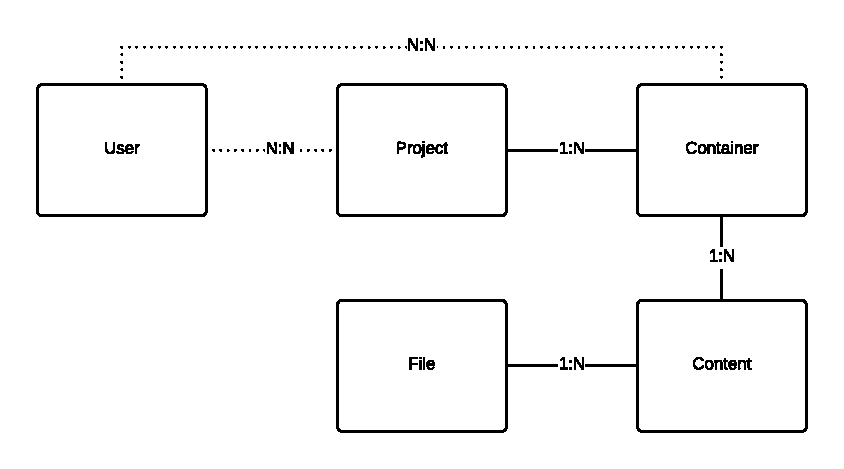
\includegraphics[scale=0.8]{relation.pdf}}
    \caption{High Level Entity Relationships}
    \label{fig:relation}
\end{figure}

\subsubsection{Content}
Content is meta data about a file and is stored in a container, it is a form of virtual file.  The
content can refer to for example an image, video or binary blob.

\subsubsection{Project}
A project is what is created to contain all content and containers related to a real project. Files
can be changed within a project and the system can contain several projects and their virtual
content are completely disjoint.

\subsubsection{Container}
A container is a virtual folder within a project which can contain content and other containers.

\subsubsection{Snapshot}
A snapshot is a read-only container from the state which the container the was in when the snapshot
was created.  A snapshot can not be updated and can only be deleted from the root of the snapshot.
Snapshots are by default stored as siblings to the container which they were made from, but they can
be contained by any container.

\subsubsection{File}
A file refers to an actual physical file. Files are stored in the database to make backup,
deployment and migration easier.

\subsubsection{User}
A user is the structure that handles people who have been granted access to the system. Access to
the system is handled by a separate service, like LDAP.

\subsection{Execution}
Java path finder was used to show that the model and plan of how to build the system was sound. The
model was built in Java with the objective of being as reduced and simple as possible, without
loosing any of the cases that needed to be covered by the model checker. As the users are mainly
going to be handled by external systems they were not included in the model.

Each collection in the persistent storage was emulated by using the built-in ConcurrentHashMap type.
Each client was represented by a thread and each action taken by the client was randomised. The id
hashes which MongoDB is using for each entity was imported from the mongo-java-driver-2.13.3 and
each object had its own id, generated in the same fashion as the real implementation is using,
randomly generated by the ObjectId class to minimise collisions that is.  Furthermore no locking or
transactions were used and the threads were running fully concurrently, without any sleep
statements. 

ConcurrentHashMap had to be used in instead of the normal HashMap, as the normal HashMaps can't be
iterated over concurrently.

JPF checked each permutation of states that the threads can end up in, the result of the run can be
seen in Listing~\ref{JPFRESULT}.

\begin{lstlisting}[label=JPFRESULT,caption=Results of JPF run]
elapsed time:       14:26:53
states:             new=160853259,
                    visited=451102505,
                    backtracked=611955764,
                    end=21640
search:             maxDepth=380,
                    constraints=0
choice generators:  thread=160853255 
                    (signal=0,
                    lock=3603938,
                    sharedRef=146989208,
                    threadApi=3,
                    reschedule=10260106), 
                    data=0

heap:               new=676056850,
                    released=435060996,
                    maxLive=655,
                    gcCycles=523950061

instructions:       11917045758
max memory:         6256MB
loaded code:        classes=111,
                    methods=2179
\end{lstlisting}


\newpage
\section{Discussion}
\subsection{Persistent Storage}
More research could have been done in the choosing of persistent storage, as mentioned in ``NoSQL:
Moving from MapReduce Batch Jobs to Event-Driven Data Collection''~\cite{KLINGSBO} many applications
that choose NoSQL databases as their persistent storage actually don't need it. This is most likely
true for Perius too, it would have been efficient enough generating the project trees from an
indexed SQL database with foreign keys. On the other hand it was quite nice having the BSON
documents for insertion as they were so similar the accepted JSON format from the REST service.
As Perius most common operations involve modifying the project tree, a graph database should have 
been researched too.

\newpage
\section{Summary}
\subsection{Conclusions}

\subsection{Future work}
\subsubsection{Access Control}
Full access control was not implemented according to the model described in ~\ref{sec:model}, it
was only implemented to check whether a user should have access to the system as a whole or not, the
implementation did not set or check any specific access rights to certain contents or containers.

\subsubsection{Front-end Refactor}
The application could be made substantially more efficient by rewriting the front-end to update
itself according to the REST response after a modification of the project tree, instead of 
re-fetching the full project tree every time a change is made.

\newpage
\bibliographystyle{ieeetr}
\bibliography{references}

\end{document}


%{{{

%What to write about
%Battle Binary
%Security features of CDN's
%What is needed by the logic, like what happens after two consecutive deletes
%
%What is needed
%* Security layers
%* snapshots
%* Virtual file structure
%* Versioning of content
%* Multi project support
%* Auth and audit logs
%* Users

%Stuff to write about:
%Modular design, every piece should be interchangeable
%LDAP - why it was used as standard AUTH

%Using copy-on-write as the sole update strategy has pros and cons. The upside is
%that it is simple to guarantee operation atomicity, and data-structure integrity. The
%downside is that performance relies on the ability to maintain large extents of free
%contiguous disk areas. In addition, random updates to a f i le tend to fragment it,
%destroying sequentiality. A good defragmentation algorithm is required; this is
%described in Section 5

%}}}
